\begin{tikzpicture}
    \begin{axis}[
        width=0.95\linewidth,
        height=0.30\textheight,
        xmin=0, xmax=6,
        xtick={0,1,2,3,4,5,6},
        xlabel={window step $t$},
        ymin=0.0, ymax=1.0,
        ytick={0.03,0.23,0.33,0.43,0.70,0.80,0.90},
        yticklabels={,$1.2$,$1.3$,$1.4$,$-1.4$,$-1.3$,$-1.2$},
        ylabel={$x$ position $p_x$},
        title style={font=\sffamily\small\bfseries},
        label style={font=\sffamily\small},
        tick label style={font=\sffamily\scriptsize, text=black!75},
        legend style={
            font=\sffamily\tiny,
            at={(0.5,0.03)},
            anchor=south,
            legend columns=2,
            draw=black!8,
            fill=white,
            fill opacity=0.92,
            text opacity=1,
            rounded corners=2pt,
            inner xsep=3pt,
            inner ysep=2pt,
        },
        axis line style={draw=black!35},
        tick style={draw=black!35},
        tick align=outside,
        grid=major,
        major grid style={draw=black!7, line width=0.25pt},
        minor tick num=0,
        every axis plot/.append style={line cap=round, line join=round},
    ]
        \addplot+[color=black!60, semithick, mark=*, mark size=1.2pt,
            mark options={fill=white, draw=black!60, line width=0.3pt}] coordinates {
            (0,0.700000000) (1,0.731935903) (2,0.764535535) (3,0.798862995)
            (4,0.835190454) (5,0.873284850) (6,0.912193598)
        };
        \addlegendentry{observed}
        \addplot+[color=blue!70!black, line width=1.8pt, mark=square*, mark size=1.5pt,
            mark options={fill=blue!70!black, draw=white, line width=0.25pt}] coordinates {
            (0,0.700000000) (1,0.731935903) (2,0.764313149) (3,0.797496517)
            (4,0.830909913) (5,0.863252654) (6,0.894049191)
        };
        \addlegendentry{selected}
        \addplot+[color=teal!70!black, line width=1.2pt, opacity=0.9,
            mark=triangle*, mark size=1.4pt,
            mark options={fill=teal!70!black, draw=white, line width=0.25pt}] coordinates {
            (0,0.700000000) (1,0.732000000) (2,0.764000000) (3,0.796000000)
            (4,0.828000000) (5,0.860000000) (6,0.892000000)
        };
        \addlegendentry{swap P2}
        \addplot+[color=orange!85!red!70!black, line width=1.2pt, opacity=0.9,
            mark=diamond*, mark size=1.3pt,
            mark options={fill=orange!85!red!70!black, draw=white, line width=0.25pt}] coordinates {
            (0,0.700000000) (1,0.731935903) (2,0.764313149) (3,0.797496517)
            (4,0.830909913) (5,0.863252654) (6,0.894049191)
        };
        \addlegendentry{swap P3}

        \addplot+[color=black!60, semithick, mark=*, mark size=1.2pt,
            mark options={fill=white, draw=black!60, line width=0.3pt}, forget plot] coordinates {
            (0,0.430000000) (1,0.399000000) (2,0.370000000) (3,0.343000001)
            (4,0.318000001) (5,0.294799939) (6,0.272399845)
        };
        \addplot+[color=blue!70!black, line width=1.8pt, mark=square*, mark size=1.5pt,
            mark options={fill=blue!70!black, draw=white, line width=0.25pt}, forget plot] coordinates {
            (0,0.430000000) (1,0.399000000) (2,0.370000000) (3,0.343000001)
            (4,0.318000001) (5,0.294799939) (6,0.272399845)
        };
        \addplot+[color=teal!70!black, line width=1.2pt, opacity=0.9,
            mark=triangle*, mark size=1.4pt,
            mark options={fill=teal!70!black, draw=white, line width=0.25pt}, forget plot] coordinates {
            (0,0.430000000) (1,0.399000000) (2,0.370000000) (3,0.343000001)
            (4,0.318000001) (5,0.294799939) (6,0.272399845)
        };
        \addplot+[color=orange!85!red!70!black, line width=1.2pt, opacity=0.9,
            mark=diamond*, mark size=1.3pt,
            mark options={fill=orange!85!red!70!black, draw=white, line width=0.25pt}, forget plot] coordinates {
            (0,0.430000000) (1,0.398000000) (2,0.366000000) (3,0.334000000)
            (4,0.302000000) (5,0.270000000) (6,0.238000000)
        };

        \draw[black!18, line width=0.45pt] (rel axis cs:0,0.50) -- (rel axis cs:1,0.50);
        \draw[black!30, line width=0.45pt] (rel axis cs:-0.005,0.47) -- (rel axis cs:0.02,0.50);
        \draw[black!30, line width=0.45pt] (rel axis cs:-0.005,0.50) -- (rel axis cs:0.02,0.53);
        \node[font=\sffamily\scriptsize, text=black!70] at (axis cs:3.3,0.71) {Player 2};
        \node[font=\sffamily\scriptsize, text=black!70] at (axis cs:3.3,0.41) {Player 3};
    \end{axis}
\end{tikzpicture}
